% Cread by Banbara on Dec. 19 2019
\documentclass[11pt,dvipdfmx]{beamer}

%%%% Packages %%%%%
 \usepackage{graphicx}
% \usepackage{amsmath,amssymb,amsthm}
% \usepackage{multirow}
% \usepackage{url}
% \usepackage{tikz}
% \usepackage{alltt}
% \usepackage{bm}
% \usepackage{listings,jlisting}
% \usepackage{listings}
% \lstset{
%  basicstyle=\ttfamily\scriptsize,
%  keepspaces=true,
%  escapechar=|,
%  columns=[l]{fullflexible}
% }

%%%% Fonts %%%%%
\renewcommand{\kanjifamilydefault}{\gtdefault}
% \usepackage{otf} % otfパッケージ
\usepackage[deluxe]{otf} 
\usepackage{txfonts} % 数式・英文ローマン体を Lxfont にする
% \usepackage[T1]{fontenc} % 8bit フォント
% \usepackage{minijs}
% \usepackage{textcomp} % 欧文フォントの追加
% \usepackage[utf8]{inputenc} % 文字コードをUTF-8

%%%% Beamer %%%%%
\usetheme{Madrid}
\useinnertheme{rectangles}
%\useoutertheme{smoothbars}
\setbeamercolor{enumerate}{fg=white, bg=black}
\usefonttheme{professionalfonts}
\setbeamertemplate{frametitle}[default][center]
\setbeamertemplate{navigation symbols}{}
% \setbeamercovered{transparent} % 好みに応じてどうぞ
\setbeamertemplate{footline}[frame number]
\setbeamercolor{page number in head/foot}{fg=black} % ページ数を表示する
% \setbeamerfont{footline}{size=\normalsize,series=\bfseries}
\setbeamerfont{footline}{size=\scriptsize,series=\mdseries}
\setbeamercolor{footline}{fg=black,bg=black}
\setbeamertemplate{blocks}[rounded][shadow=true]
\setbeamertemplate{items}[ball]
% \setbeamertemplate{enumerate items}[default]
% \setbeamerfont{alerted text}{series=\bfseries}

%%%% My macro %%%%%
%%%%%%%%%%%%%%%%%%%%%%%%%%%%%%%%%%%%%%%%%%%%%%%%%%%%%%%%%%%%%%%%
% User-defined Macro
%%%%%%%%%%%%%%%%%%%%%%%%%%%%%%%%%%%%%%%%%%%%%%%%%%%%%%%%%%%%%%%%
\newcommand{\compress}{\itemsep0pt\parsep0pt\parskip0pt\partopsep0pt}
% \newcommand{\compress}{\itemsep1pt plus1pt\parsep0pt\parskip0pt}
% \newcommand{\code}[1]{\lstinline[basicstyle=\ttfamily]{#1}}
\newcommand{\gringo}{\textit{gringo}}
\newcommand{\clasp}{\textit{clasp}}
\newcommand{\clingo}{\textit{clingo}}
\newcommand{\teaspoon}{\textit{teaspoon}}
\newcommand{\sat}{\textsf{SAT}}
\newcommand{\unsat}{\textsf{UNSAT}}
% \newcommand{\web}[2]{\href{#1}{#2\ \raisebox{-0.15ex}{\beamergotobutton{Web}}}}
% \newcommand{\doi}[2]{\href{#1}{#2\ \raisebox{-0.15ex}{\beamergotobutton{DOI}}}}
% \newcommand{\weblink}[1]{\web{#1}{#1}}
% \newcommand{\imp}{\mathrel{\Rightarrow}}
% \newcommand{\Iff}{\mathrel{\Leftrightarrow}}
% \newcommand{\mybox}[1]{\fbox{\rule[.2cm]{0cm}{0cm}\mbox{${#1}$}}}
% \newcommand{\mycbox}[2]{\tikz[baseline]\node[fill=#1!10,anchor=base,rounded corners=2pt] () {#2};}
% \newcommand{\naf}[1]{\ensuremath{{\sim\!\!{#1}}}}
% \newcommand{\head}[1]{\ensuremath{\mathit{head}(#1)}}
% \newcommand{\body}[1]{\ensuremath{\mathit{body}(#1)}}
% \newcommand{\atom}[1]{\ensuremath{\mathit{atom}(#1)}}
% \newcommand{\poslits}[1]{\ensuremath{{#1}^+}}
% \newcommand{\neglits}[1]{\ensuremath{{#1}^-}}
% \newcommand{\pbody}[1]{\poslits{\body{#1}}}
% \newcommand{\nbody}[1]{\neglits{\body{#1}}}
% \newcommand{\Cn}[1]{\ensuremath{\mathit{Cn}(#1)}}
% \newcommand{\reduct}[2]{\ensuremath{#1^{#2}}}
% \newcommand{\OK}{\mbox{\textcolor{green}{\Pisymbol{pzd}{52}}}}
% \newcommand{\KO}{\mbox{\textcolor{red}{\Pisymbol{pzd}{56}}}}
% \newcommand{\code}[1]{\lstinline[basicstyle=\ttfamily]{#1}}
% \newcommand{\lw}[1]{\smash{\lower2.ex\hbox{#1}}}
\newcommand{\llw}[1]{\smash{\lower3.ex\hbox{#1}}}

\newenvironment{tableC}{%
  \scriptsize
  \renewcommand{\arraystretch}{0.9}
  \tabcolsep = 0.6mm
  % \begin{tabular}[t]{p{6mm}|rlr|rlr|rlr|rlr|rlr}\hline
  %   \multicolumn{1}{l|}{\llw{問題   }} &
  \begin{tabular}[t]{l|rlr|rlr|rlr|rlr|rlr}\hline
    \multicolumn{1}{l|}{\llw{問題}} &
    \multicolumn{3}{c|}{UD1} &
    \multicolumn{3}{c|}{UD2} &
    \multicolumn{3}{c|}{UD3} &
    \multicolumn{3}{c|}{UD4} &
    \multicolumn{3}{c}{UD5} \\
    & 
    \multicolumn{1}{c}{既知の} & & \multicolumn{1}{c|}{ASP} & 
    \multicolumn{1}{c}{既知の} & & \multicolumn{1}{c|}{ASP} & 
    \multicolumn{1}{c}{既知の} & & \multicolumn{1}{c|}{ASP} & 
    \multicolumn{1}{c}{既知の} & & \multicolumn{1}{c|}{ASP} & 
    \multicolumn{1}{c}{既知の} & & \multicolumn{1}{c}{ASP} \\
    & 
    ベスト & &  & 
    ベスト & &  & 
    ベスト & &  & 
    ベスト & &  & 
    ベスト & &  \\
    \hline
  }{%
    \hline
  \end{tabular}
}

%%%%%%%%%%%%%%%%%%%%%%%%%%%%%%%%%%%%%%%%%%%%%%%%%%%%%%%%%%%%%%%%%%%%%%%
\title{解集合プログラミングを用いた\\時間割問題の解法に関する研究}
\author{桑原 和也 (081630434)}
\institute{名古屋大学工学部電気電子・情報学科情報コース}
\date{番原研究室中間発表\\2019年12月20日}

\begin{document}
\maketitle
%%%%%%%%%%%%%%%%%%%%%%%%%%%%%%%%%%%%%%%%%%%%%%%%%%%%%%%%%%%%%%%%%%%%%%%
\begin{frame}{時間割問題}
  \begin{block}{}\centering
    求解困難な組合せ最適化問題の一種である.
  \end{block}
  \begin{itemize}
    % \item 現状では,実行可能で質の高い時間割を作成するために
    %   多くの人間の労力が費やされている.
  \item 時間割に関する国際会議 PATAT および
    \alert{\bf 国際的な時間割競技会}が開催され,
    時間割ソルバーの性能向上に貢献している.
    \begin{itemize}
    \item 教育時間割
      \begin{itemize}
      \item \alert{\bf カリキュラムベース・コース時間割 (CB-CTT)}
      \item ポストエンロールメント・コース時間割
      \item 試験時間割
      \end{itemize}
    \item 輸送時間割
    \item 従業員時間割
    \item スポーツ時間割
    \end{itemize}
  \item 本発表では,最も研究が盛んな CB-CTT を対象とする.
  \item CB-CTT は,以下のように定式化される.
    \begin{itemize}
    \item 必ず満たすべき\structure{\bf ハード制約}と,
      できるだけ満たしたい\structure{\bf 重み付きソフト制約}から構成される.
    \item 違反するソフト制約の重み (ペナルティ) の総和の最小化が目的.
    \end{itemize}
  \end{itemize}
\end{frame}
%%%%%%%%%%%%%%%%%%%%%%%%%%%%%%%%%%%%%%%%%%%%%%%%%%%%%%%%%%%%%%%%%%%%%%%
\begin{frame}{解集合プログラミング(Answer Set Programming; ASP)}
  \begin{itemize}
  \item \structure{\bf ASP言語}は,一階論理に基づく知識表現言語の一種である.
  \item \structure{\bf ASPシステム}は,安定モデル意味論~[Gelfond and Lifschitz '88]
    に基づく解集合を計算するシステムである.
  \item 近年,SAT技術を利用した高速なASPシステムが開発され,ロボット工学,
    システム検証,システム生物学など
    様々な分野への実用的応用が急速に拡大している.
  \end{itemize}
  \begin{exampleblock}{組合せ最適化問題に対してASPを用いる利点}
    \begin{itemize}
    \item ASP言語の高い表現力により,各制約を表現する論理プログラムを
      モジュール化して容易に切り替え可能である.
    \item 系統的探索 (分枝限定法) なので,解の最適性を保証できる.
%    \item 様々な最適化手法や探索ヒューリスティックスを試せる.
    \item 探索ヒューリスティックスを試せる.
      \begin{itemize}
      \item 探索時に優先的に割り当てる値を指定できる.
      \end{itemize}
%    \item Python インターフェースを利用して,メタヒューリスティックスを実装できる.
    \end{itemize}
  \end{exampleblock}
\end{frame}
%%%%%%%%%%%%%%%%%%%%%%%%%%%%%%%%%%%%%%%%%%%%%%%%%%%%%%%%%%%%%%%%%%%%%%%
\begin{frame}{CB-CTT に対する既存ASP解法の問題点}
  \begin{itemize}
  \item ASP による解法は,
    最も成功した ASP 応用事例の一つとして知られている~[Banbara+ 2013, 2016, 2018].
    \begin{itemize}
    \item ベンチマーク問題305問のうち,
      179問で既知の最良値と同じかより良い値が求められている.
    \end{itemize}
  \item 系統的探索であることを活かして,最適値が未知であった問題の最適値決定にも成功している.
    \begin{itemize}
    \item 305問中51問で最適値が求められている.
    \end{itemize}
  \end{itemize}
  \begin{alertblock}{既存ASP解法の問題点}
    \begin{itemize}
    \item ソフト制約が多く含まれるような問題において,
      局所的探索より性能が劣っている場合がみられる.
    % \item 既知の最良値との比の平均値は
    %   \begin{itemize}
    %   \item ソフト制約が少ない問題集 (UD1) では $+12.12\%$,
    %   \item ソフト制約が多い問題集 (UD5) では $+114.50\%$ である.
    %   \end{itemize}
    \end{itemize}
  \end{alertblock}
\end{frame}
%%%%%%%%%%%%%%%%%%%%%%%%%%%%%%%%%%%%%%%%%%%%%%%%%%%%%%%%%%%%%%%%%%%%%%%
\begin{frame}{研究目的}
  \begin{block}{先行研究}
    我々の研究室では,
    系統的探索と局所的探索を組み合わせた手法
    \alert{Large Neighborhood Prioritized Search (LNPS)} [坡山ほか '18]を提案し,
    応用事例の蓄積を行なっている.
  \end{block}

  \begin{alertblock}{研究目的}
    LNPS を ASP 上に実装し,CB-CTT に適用・評価する.
  \end{alertblock}

  \begin{block}{研究内容}
    \begin{enumerate}
    \item LNPS の性能に重要な役割を果たす destroy 演算について,
      CB-CTT に適した3種類の手法を実装した.
    \item CB-CTT に対する実験・評価
    \end{enumerate}
  \end{block}
\end{frame}
%%%%%%%%%%%%%%%%%%%%%%%%%%%%%%%%%%%%%%%%%%%%%%%%%%%%%%%%%%%%%%%%%%%%%%%
\begin{frame}{LNPS (Large Neighborhood Prioritized Search) [坡山'18]}
  \begin{block}{\small LNPS のアルゴリズム}
    \begin{enumerate}
      \compress
      \item 初期解を $x$ と置き,最良解 $x* := x$ とする.
      \item 以下の destroy と re-searchで $x$ から得られた解を $x_t$ と置く.
      \begin{itemize}
        \compress
        \item \alert{\bf destroy} は $x$ から値割当ての一部を取り消し $x'$ とする.
        \item re-search は $x'$ の\structure{値割当てをなるべく維持したまま再探索}する.
      \end{itemize}
      \item 更新条件を満たしていたら $x := x_t$ とする.
      \begin{itemize}
        \item 例えば「$x_t$ が $x$ より改善された解なら」という更新条件を用いる.
      \end{itemize}
      \item $x_t$ が最良解 $x*$ より改善された解なら,$x* := x_t$ とする.
      \item 終了条件が満たされるまで,2〜4 を繰り返す.
      \begin{itemize}
        \item 例えば繰り返し回数や制限時間などを終了条件に用いる.
      \end{itemize}
      \item 最良解 $x*$ を返す.
    \end{enumerate}
  \end{block}

  \begin{itemize}
  \item 運搬経路問題 (Vehicle Routing Problem)
    等に対して有効性が示されている
    Large Neighborhood Search (LNS) [Shaw '98, Ropke and Pisinger '10]
    をベース
  \item 問題に応じて,\alert{\bf 適切な destroy 演算を設計}することが重要.
  \end{itemize}
\end{frame}
%%%%%%%%%%%%%%%%%%%%%%%%%%%%%%%%%%%%%%%%%%%%%%%%%%%%%%%%%%%%%%%%%%%%%%%
\begin{frame}{実装した destroy 演算}
  \small CB-CTT に対する既存の destroy 演算を参考に,3種類の手法を実装した.
  \begin{block}{\small destroy 演算}
  \begin{enumerate}
  \item \small R-$n$\%(Random $n$\% destruction)
  \begin{itemize}
   \item \scriptsize 値割り当てから,ランダムに$n$\%選択して取り消す.
   \item \scriptsize 今回の実装では$n$として0,10,20の3種類を選択した.
  \end{itemize}
  \item \small R-dp(Random day-period destruction)
   \begin{itemize}
    \item \scriptsize ランダムにday(曜日)とperiod(時限)を選択し,選んだ曜日の選んだ時限に割り当てられている値割り当てを取り消す.
    \item \scriptsize この destroy 演算は,割り当てられるroom(教室)の変更を促進させ, roomに関する制約へのペナルティを改善することを狙いとしている.
   \end{itemize}
  \item \small R-dr(Random day-room destruction)
   \begin{itemize}
    \item \scriptsize ランダムに day と room を選択し,選んだ曜日の選んだ教室に割り当てられている値割り当てを取り消す.
    \item \scriptsize この destroy 演算は,割り当てられる period の変更を促進させ, period に関する制約へのペナルティを改善することを狙いとしている.
   \end{itemize}
  \end{enumerate}
  \end{block}
  \begin{itemize}
   \item \small R-dpとR-drでは,取り消すことのできる値割り当てが存在しなければ,存在するようになるまでランダムな選択を繰り返す.
  \end{itemize}
 \end{frame}
%%%%%%%%%%%%%%%%%%%%%%%%%%%%%%%%%%%%%%%%%%%%%%%%%%%%%%%%%%%%%%%%%%%%%%%
\begin{frame}{実験概要}
  \begin{itemize}
    \item 実装した解法の性能を評価するために比較実験を行った.
    \begin{enumerate}
      \item 既存 ASP 解法 (系統的探索のみ)~[Banbara+ 2018]
      \item 実装解法1 (LNPS + R-0\% / R-10\% / R-20\%)
      \item 実装解法2 (LNPS + R-dp)
      \item 実装解法3 (LNPS + R-dr)
    \end{enumerate}
    \item CB-CTTベンチマーク問題 (全21問)
    \begin{itemize}
      \item ソフト制約が多い問題集 (UD5) を用いる.
    \end{itemize}
    \item ASP システム:\textit{clingo-5.4.0}
    \item 既存ASP解法の制限時間は1時間
   \item 実装解法1〜3では、制限時間30分の既存ASPの解を初期解とし,各 destroy 演算を1回行った後,10分を制限時間とした.
  \end{itemize}
\end{frame}
%%%%%%%%%%%%%%%%%%%%%%%%%%%%%%%%%%%%%%%%%%%%%%%%%%%%%%%%%%%%%%%%%%%%%%% 
\begin{frame}{実験結果 (1)}
 \centering
 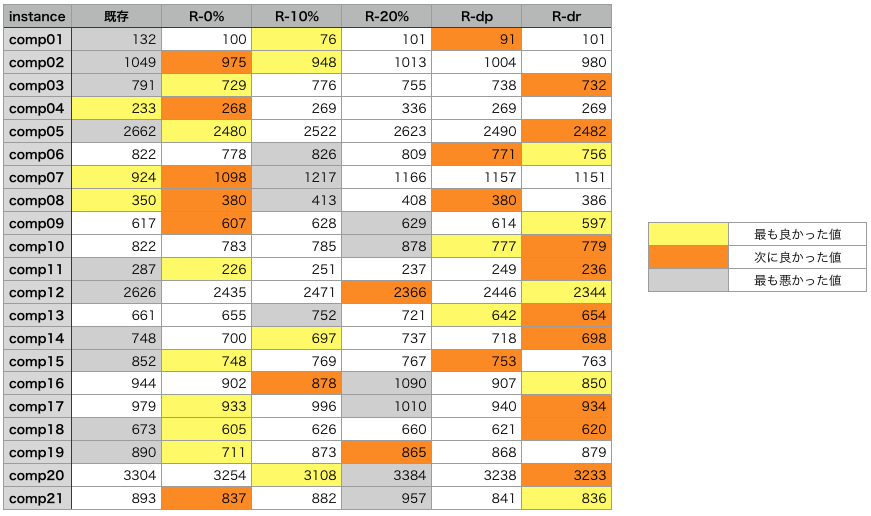
\includegraphics[width=10cm]{pic/opt.png}
 \begin{itemize}
 \item \small R-0\%は黄が7問,燈が6問となり,R-drは黄が5問,燈が9問と両者が特に良い結果を示した.
 \item \small 既存解法は黄が3問,灰が10問となり,R-20\%は燈が2問,灰が6問と両者が特に悪い結果を示した.
 \end{itemize}
\end{frame}
%%%%%%%%%%%%%%%%%%%%%%%%%%%%%%%%%%%%%%%%%%%%%%%%%%%%%%%%%%%%%%%%%%%%%%%
\begin{frame}{実験結果 (2)}
 \scriptsize 合計講義数(割り当てる必要のある講義数)で降順にソート
  \centering
  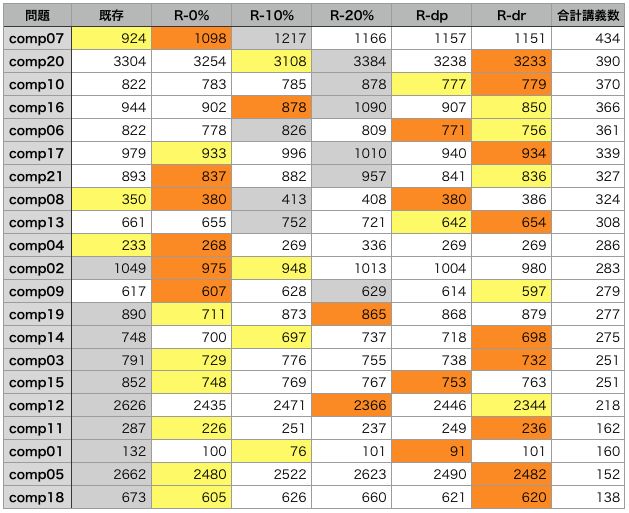
\includegraphics[width=7cm]{pic/lecture_sort.png}
  \begin{itemize}
  \item \small 講義数の少ない問題では既存解法が悪く.講義数の多い問題ではR-10\%やR-20\%が悪いという傾向が確認できた.
 \item \small R-dp,R-drの結果は講義数に依存するという傾向は確認できなかった.
  \end{itemize}
\end{frame}
%%%%%%%%%%%%%%%%%%%%%%%%%%%%%%%%%%%%%%%%%%%%%%%%%%%%%%%%%%%%%%%%%%%%%%%
\begin{frame}{まとめ}
  \small LNPS を CB-CTT に適用し,その有効性を評価するために以下を行なった.
  \begin{enumerate}
  \item \small 既存の destroy 演算を参考に,CB-CTT に対する 3種類の destroy
    演算を実装した.
    \begin{itemize}
    \item \footnotesize R-$n$\%は,他の組み合わせ最適化問題にも適用可能である.
    \end{itemize}
  \item \small CB-CTT のソフト制約が多い問題集 (UD5) での実験・評価を行った.
    \begin{itemize}
    \item \footnotesize 既存解法に比べ,R-0\%は最も良い解を示す問題が多く,次いでR-dr,R-dpで良い解が得られた.
   \item \footnotesize R-10\%,R-20\%では,他の手法に比べて既存解法より悪い解が得られる問題数が多かった.
    \end{itemize}
  \end{enumerate}
    
  \begin{alertblock}{\small 今後の課題}
    \begin{itemize}
    \item \small より良い destroy/re-search の方法の考案・評価
    \begin{itemize}
    \item \footnotesize 問題のサイズによる適切なdestroyの割合の決定
   \item \footnotesize 問題のサイズによらないdestroy演算の実装
    \end{itemize}
    \item 他の時間割問題,および組合せ最適化問題での実験
    \end{itemize}
  \end{alertblock}
\end{frame}
%%%%%%%%%%%%%%%%%%%%%%%%%%%%%%%%%%%%%%%%%%%%%%%%%%%%%%%%%%%%%%%%%%%%%%%
% 補助スライド
\appendix
%%%%%%%%%%%%%%%%%%%%%%%%%%%%%%%%%%%%%%%%%%%%%%%%%%%%%%%%%%%%%%%%%%%%%%%
\begin{frame}{制約と問題集 (カリキュラムベース・コース時間割)}
  % \begin{itemize}
  % \item \structure{シナリオ}とはソフト制約の集合である.
  %   % \item ITC2007競技会ではUD2が使用された.
  % \end{itemize}
  \begin{block}{}\small
    \begin{center}
      \begin{tabular}{l|ccccc}%\hline
        制約                      &  UD1  &  UD2  &  UD3  &  UD4  &  UD5  \\
        \hline
        $H_1$. Lectures           &  H    &  H    &  H    &  H    &  H    \\
        $H_2$. Conflicts          &  H    &  H    &  H    &  H    &  H    \\
        $H_3$. RoomOccupancy      &  H    &  H    &  H    &  H    &  H    \\
        $H_4$. Availability       &  H    &  H    &  H    &  H    &  H    \\
        $S_1$. RoomCapacity       &  1    &  1    &  1    &  1    &  1    \\
        $S_2$. MinWorkingDays     &  5    &  5    &  -    &  1    &  5    \\
        $S_3$. IsolatedLectures   &  1    &  2    &  -    &  -    &  1    \\
        $S_4$. Windows            &  -    &  -    &  4    &  1    &  2    \\
        $S_5$. RoomStability      &  -    &  1    &  -    &  -    &  -    \\
        $S_6$. StudentMinMaxLoad  &  -    &  -    &  2    &  1    &  2    \\
        $S_7$. TravelDistance     &  -    &  -    &  -    &  -    &  2    \\
        $S_8$. RoomSuitability    &  -    &  -    &  3    &  H    &  -    \\
        $S_9$. DoubleLectures     &  -    &  -    &  -    &  1    &  -  
      \end{tabular}
    \end{center}
  \end{block}
\end{frame}
%%%%%%%%%%%%%%%%%%%%%%%%%%%%%%%%%%%%%%%%%%%%%%%%%%%%%%%%%%%%%%%%
\begin{frame}{CB-CTT に対する既存ASPの結果~[Banbara+ '18]}
  \centering
  \scriptsize
  \begin{tableC}
    \texttt{comp01} & 4 & $=$ & 4 & 5 & $=$ & 5 & 8 & $=$ & 8 & 6 &  & 9 & 11 &  & 19\\
\texttt{comp02} & 12 & $=^*$ & \alert{12} & 24 & $=^*$ & \alert{24} & 12 & $=^*$ & \alert{12} & 26 &  & 55 & 130 &  & 231\\
\texttt{comp03} & 38 & & 53 & 64 &  & 109 & 25 &  & 47 & 362 &  & 405 & 142 &  & 204\\
\texttt{comp04} & 18 & $=$ & 18 & 35 & $=$ & 35 & 2 & $=^*$ & \alert{2} & 13 & $=^*$ & \alert{13} & 59 & $>^*$ & \alert{49}\\
\texttt{comp05} & 219 &  & 504 & 284 &  & 624 & 264 &  & 556 & 260 &  & 459 & 570 &  & 1081 \\
\texttt{comp06} & 14 & $=^*$ & \alert{14} & 27 & $=$ & 27 & 8 & $=^*$ & \alert{8} & 15 & $>^*$ & \alert{9} & 85 &  & 88 \\
\texttt{comp07} & 3 & $=$ & 3 & 6 & $=$ & 6 & 0 & $=$ & 0 & 3 & $=^*$ & \alert{3} & 42 &  & 256 \\
\texttt{comp08} & 19 & $=$ & 19 & 37 & $=$ & 37 & 2 & $=^*$ & \alert{2} & 15 & $=^*$ & \alert{15} & 62 & $>^*$ & \alert{55} \\
\texttt{comp09} & 54 &  & 63 & 96 &  & 169 & 8 & $=^*$ & \alert{8} & 38 &  & 50 & 150 &  & 196 \\
\texttt{comp10} & 2 & $=$ & 2 & 4 & $=$ & 4 & 0 & $=$ & 0 & 3 & $=^*$ & \alert{3} & 72 &  & 73 \\
\texttt{comp11} & 0 & $=$ & 0 & 0 & $=$ & 0 & 0 & $=$ & 0 & 0 & $=$ & 0 & 0 & $=$ & 0 \\
\texttt{comp12} & 239 &  & 343 & 294 &  & 456 & 51 &  & 114 & 99 &  & 388 & 483 &  & 1135 \\
\texttt{comp13} & 32 & $>^*$ & \alert{31} & 59 & $=$ & 59 & 22 &  & 50 & 41 &  & 111 & 148 & $>$ & 147 \\
\texttt{comp14} & 27 & $=^*$ & \alert{27} & 51 & $=$ & 51 & 0 & $=$ & 0 & 16 & $>^*$ & \alert{14} & 95 & $>*$ & \alert{67} \\
\texttt{comp15} & 38 &  & 53 & 62 &  & 109 & 16 &  & 22 & 30 &  & 68 & 176 &  & 254 \\
\texttt{comp16} & 11 & $=^*$ & \alert{11} & 18 & $=$ & 18 & 4 & $=^*$ & \alert{4} & 7 & $=^*$ & \alert{7} & 96 &  & 438 \\
\texttt{comp17} & 30 & $=^*$ & \alert{30} & 56 & $=$ & 56 & 12 & $=^*$ & \alert{12} & 26 & $>^*$ & \alert{21} & 155 &  & 352 \\
\texttt{comp18} & 34 &  & 48 & 61 &  & 81 & 0 & $=$ & 0 & 27 &  & 46 & 137 &  & 228 \\
\texttt{comp19} & 32 & $>^*$ & \alert{29} & 57 & $=$ & 57 & 24 &  & 32 & 32 &  & 82 & 125 &  & 283 \\
\texttt{comp20} & 2 & $=$ & 2 & 4 & $=$ & 4 & 0 & $=$ & 0 & 9 & $>^*$ & \alert{3} & 124 &  & 704 \\
\texttt{comp21} & 43 &  & 94 & 74 &  & 124 & 6 & $=$ & 6 & 36 &  & 76 & 151 &  & 166 \\
% \texttt{DDS1} & 38 & $=^*$ & 38 & 48 & $=$ & 48 & 2393 &  & 6036 & 2278 & $=$ & 2278 & 1831 &  & 4662 \\
% \texttt{DDS2} & 0 & $=$ & 0 & 0 & $=$ & 0 & 120 &  & 379 & 76 &  & 139 & 64 &  & 150 \\
% \texttt{DDS3} & 0 & $=$ & 0 & 0 & $=$ & 0 & 22 & $=$ & 22 & 11 & $=$ & 11 & 22 & $=$ & 22 \\
% \texttt{DDS4} & 16 &  & 19 & 17 &  & 33 & 54 &  & 912 & 124 &  & 1825 & 96 &  & 2384 \\
% \texttt{DDS5} & 0 & $=$ & 0 & 0 & $=$ & 0 & 54 &  & 117 & 163 &  & 488 & 88 & $>^*$ & 76 \\
% \texttt{DDS6} & 0 & $=$ & 0 & 0 & $=$ & 0 & 0 & $=$ & 0 & 0 & $=$ & 0 & 96 &  & 509 \\
% \texttt{DDS7} & 0 & $=$ & 0 & 0 & $=$ & 0 & 30 &  & 408 & 21 &  & 506 & 52 &  & 66 \\
% \texttt{EA01} & 55 & $=^*$ & 55 & 65 & $=^*$ & 65 & 102 &  & 110 & 67 &  & 88 & 196 &  & 313 \\
% \texttt{EA02} & 0 & $=$ & 0 & 0 & $=$ & 0 & 96 &  & 263 & 41 &  & 262 & 128 &  & 166 \\
% \texttt{EA03} & 1 & $=$ & 1 & 2 & $=$ & 2 & 50 &  & 234 & 6936 & $>$ & 816 & 90 &  & 661 \\
% \texttt{EA04} & 0 & $=$ & 0 & 0 & $=$ & 0 & 18 &  & 21 & 9 &  & 695 & 18 & $=$ & 18 \\
% \texttt{EA05} & 0 & $=$ & 0 & 0 & $=$ & 0 & 14 & $=$ & 14 & 7 &  & 8 & 14 & $=$ & 14 \\
% \texttt{EA06} & 5 & $=^*$ & 5 & 5 & $=^*$ & 5 & 42 &  & 156 & 27 &  & 336 & 99 &  & 263 \\
% \texttt{EA07} & 0 & $=$ & 0 & 0 & $=$ & 0 & 206 &  & 1822 & 3884 & $>$ & 1122 & 205 &  & 511 \\
% \texttt{EA08} & 0 & $=$ & 0 & 0 & $=$ & 0 & 40 &  & 48 & 20 &  & 82 & 40 & $=$ & 40 \\
% \texttt{EA09} & 2 & $=^*$ & 2 & 4 & $=^*$ & 4 & 40 & $=$ & 40 & 22 &  & 27 & 48 & $=$ & 48 \\
% \texttt{EA10} & 0 & $=$ & 0 & 0 & $=$ & 0 & 4 &  & 141 & 19 &  & 573 & 93 &  & 245 \\
% \texttt{EA11} & 0 & $=$ & 0 & 0 & $=$ & 0 & 36 &  & 52 & 19 &  & 22 & 45 & $>$ & 40 \\
% \texttt{EA12} & 2 & $=^*$ & 2 & 4 & $=^*$ & 4 & 22 &  & 38 & 12 &  & 24 & 27 &  & 28 \\
% \texttt{erlangen2011\_2} & $n.a$ & $>$ & 3909 & 4670 &  & 11167 & $n.a$ & $>$ & 12790 & $n.a$ & $>$ & 6097  & $n.a$ & $>$ & 12353 \\
% \texttt{erlangen2012\_1} & $n.a$ & $>$ & 7207 & 7862 &  & 12563 & $n.a$ & $>$ & 18875 & $n.a$ & $>$ & 14212 & $n.a$ & $>$ & 28236 \\
% \texttt{erlangen2012\_2} & $n.a$ & $>$ & 12140 & 8813 &  & 23817 &  $n.a$ & $>$ & 29169  & $n.a$ & $>$ & 18741  & $n.a$ & $>$ & 37103 \\
% \texttt{erlangen2013\_1} & $n.a$ & $>$ & 9415 & 7359 &  & 17730 &  $n.a$ & $>$ & 20192 & $n.a$ & $>$ & 8201  & $n.a$ & $>$ & 28997 \\
% \texttt{erlangen2013\_2} & $n.a$ & $>$ & 9901 & 8150 &  & 19839 & $n.a$ & $>$ & 23285 & $n.a$ & $>$ & 12682 & $n.a$ & $>$ & 30533\\
% \texttt{erlangen2014\_1} & $n.a$ & $>$ & 9205 & 5981 &  & 18395 & $n.a$ & $>$ & 20286 & $n.a$ & $>$ & 8048  & $n.a$ & $>$ & 28655 \\
% \texttt{test1} & 212 &  & 328 & 224 &  & 404 & 200 &  & 299 & 208 &  & 413 & 232 &  & 532 \\
% \texttt{test2} & 8 & $=$ & 8 & 16 & $=$ & 16 & 0 & $=$ & 0 & 4 & $=^*$ & 4 & 20 & $=^*$ & 20 \\
% \texttt{test3} & 35 & $=$ & 35 & 67 &  & 113 & 18 & $=^*$ & 18 & 18 & $>^*$ & 17 & 97 & $>^*$ & 68 \\
% \texttt{test4} & 27 &  & 91 & 73 &  & 156 & 12 & $>^*$ & 6 & 33 &  & 37 & 166 &  & 278 \\
% \texttt{toy} & 0 & $=$ & 0 & 0 & $=$ & 0 & 0 & $=$ & 0 & 0 & $=$ & 0 & 0 & $=$ & 0 \\
% \texttt{Udine1} & 0 & $=$ & 0 & 0 & $=$ & 0 & 128 &  & 426 & 64 &  & 427 & 138 &  & 234 \\
% \texttt{Udine2} & 4 & $=$ & 4 & 8 & $=^*$ & 8 & 34 &  & 322 & 30 &  & 320 & 81 &  & 131 \\
% \texttt{Udine3} & 0 & $=$ & 0 & 0 & $=$ & 0 & 24 &  & 88 & 19 &  & 67 & 54 & $>^*$ & 37 \\
% \texttt{Udine4} & 35 & $=$ & 35 & 64 & $=$ & 64 & 24 & $=^*$ & 24 & 31 & $=^*$ & 31 & 108 & $>^*$ & 106 \\
% \texttt{Udine5} & 0 & $=$ & 0 & 0 & $=$ & 0 & 44 &  & 338 & 23 &  & 145 & 47 &  & 78 \\
% \texttt{Udine6} & 0 & $=$ & 0 & 0 & $=$ & 0 & 36 &  & 76 & 18 &  & 50 & 38 & $>$ & 36 \\
% \texttt{Udine7} & 0 & $=$ & 0 & 0 & $=$ & 0 & 64 &  & 94 & 32 &  & 62 & 64 & $=$ & 64 \\
% \texttt{Udine8} & 16 & $=^*$ & 16 & 31 & $>^*$ & 29 & 42 &  & 297 & 31 &  & 149 & 88 &  & 170 \\
% \texttt{Udine9} & 18 & $=$ & 18 & 21 & $=^*$ & 21 & 28 &  & 62 & 23 &  & 91 & 70 & $>$ & 56 \\
% \texttt{UUMCAS\_A131} & $n.a$ & $>$ & 776 & 708 & $>$ & 274 & $n.a$ & $>$ & 28088 & $n.a$ & $>$ & 10955 & $n.a$ & $>$ & 19699 \\
%%% Local Variables:
%%% mode: latex
%%% TeX-master: "../paper"
%%% End:
  \end{tableC}
\end{frame}
%%%%%%%%%%%%%%%%%%%%%%%%%%%%%%%%%%%%%%%%%%%%%%%%%%%%%%%%%%%%%%%%%%%%%%%
\begin{frame}{LNS (Large Neighborhood Search)}
  \begin{block}{LNS のアルゴリズム~[Pisinger 2010]}
    \begin{enumerate}
      \compress
      \item 初期解を $x$ と置き,最良解 $x* := x$ とする.
      \item 以下のdestroy と repairで $x$ から得られた解を $x_t$ と置く.
      \begin{itemize}
        \compress
%        \item destroy は $x$ から一定の割合でランダムに値割当てを選択し $x'$ とする.
      \item destroy は $x$ から値割当ての一部を取り消し $x'$ とする.
      \item repair は $x'$ の\alert{値割当てを変化させずに解を再構築}する.
      \end{itemize}
      \item 更新条件を満たしていたら $x := x_t$ とする.
      \begin{itemize}
        \item 例えば「$x_t$ が $x$ より改善された解なら」という更新条件を用いる.
      \end{itemize}
      \item $x_t$ が最良解 $x*$ より改善された解なら,$x* := x_t$ とする.
      \item 終了条件が満たされるまで,2〜4 を繰り返す.
      \begin{itemize}
        \item 例えば繰り返し回数や制限時間などを終了条件に用いる.
      \end{itemize}
      \item 最良解 $x*$ を返す.
    \end{enumerate}
  \end{block}
  \begin{itemize}
    \item 再構築した解 $x_t$ では,取り消された変数に対してのみ再割当てが行われ,$x'$ の値割当ては変化しない.
    \item VRP (Vehicle Routing Problem) など,比較的独立した複数の部分問題に分割できる場合に
          良い性能を示すことが報告されている.
  \end{itemize}
\end{frame}
%%%%%%%%%%%%%%%%%%%%%%%%%%%%%%%%%%%%%%%%%%%%%%%%%%%%%%%%%%%%%%%%%%%%%%%
% \begin{frame}{LNPS (Large Neighborhood Prioritized Search)}
%   LNSでは,取り消された変数に対してのみ再割当てが行われ,他の変数の値は変化しない.
%   \begin{block}{LNPS}
%     % \alert{値割当てをなるべく維持したままでの再探索}で解の再構築の操作を
%     % 置き換えることにより,取り消されなかった変数への再割当てを許す.
%     解の再構築の操作を,
%     \alert{値割当てをなるべく維持したままでの再探索}に置き換えることで,
%     取り消されなかった変数への再割当てを許す.
%     \begin{itemize}
%       \item ASPでは,解の再構築は系統的探索で行うことができる.
%       \begin{itemize}
%         \item 系統的探索の場合,再構築で値割り当てを固定する必要はない.
%         \item ASPシステムは学習節を保持するので,再探索のコストが小さい.
%       \end{itemize}
%       \item どの割当てに対してdestroyを行うかに依存しすぎない探索を行える.
%       \item 値割当てをなるべく維持したままでの再探索が自然に実現できる.
%       \begin{itemize}
%         \item ASP の探索ヒューリスティックスの機能を利用する.
%       \end{itemize}
%     \end{itemize}
%   \end{block}
% \end{frame}
%%%%%%%%%%%%%%%%%%%%%%%%%%%%%%%%%%%%%%%%%%%%%%%%%%%%%%%%%%%%%%%%%%%%%%%
\begin{frame}{既存解法(制限時間30分)からの解の改善率}
  \centering
 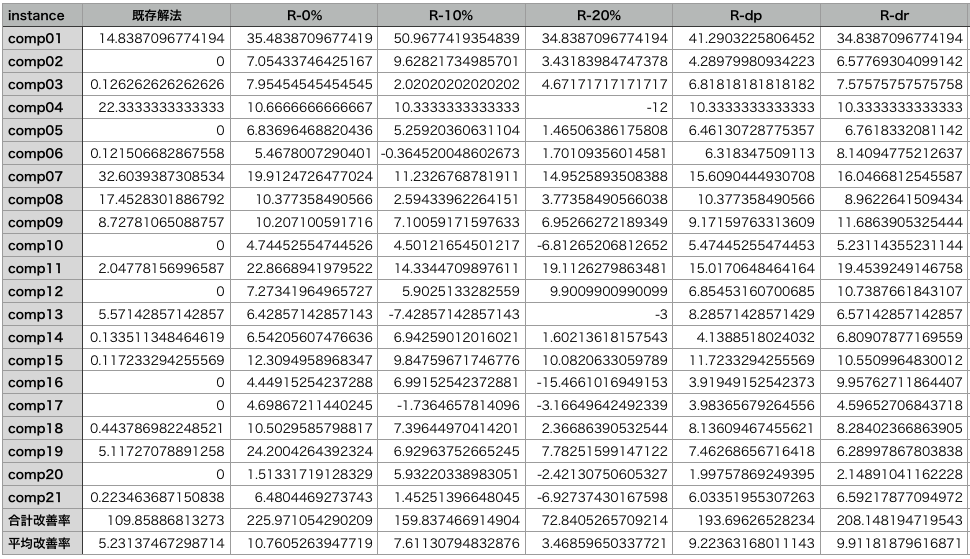
\includegraphics[width=12cm]{pic/improve.png}
\end{frame}

\begin{frame}{初期解と既存の最良値を含めた比較}
  \centering
 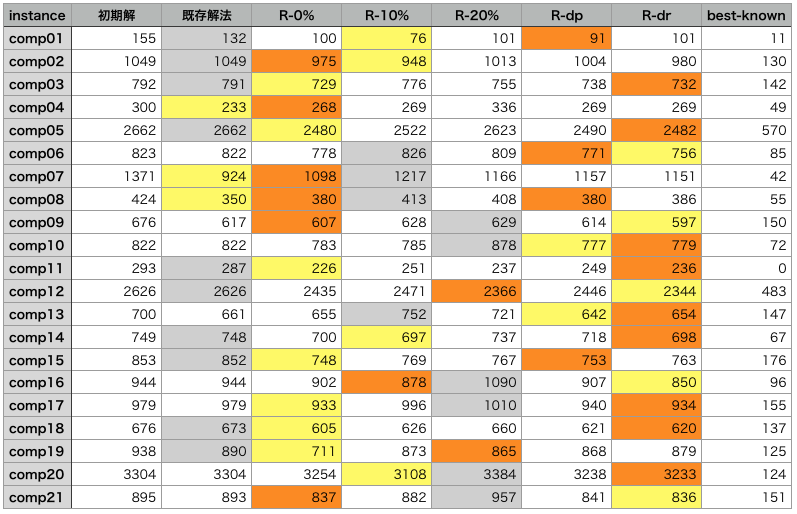
\includegraphics[width=12cm]{pic/comp.png}
\end{frame}

\end{document}

%%% Local Variables:
%%% mode: latex
%%% TeX-master: t
%%% End:
